\section{Durchführung}
\label{sec:Durchfuehrung}
\subsection{Aufbau}
    \begin{figure}[h]
        \center
        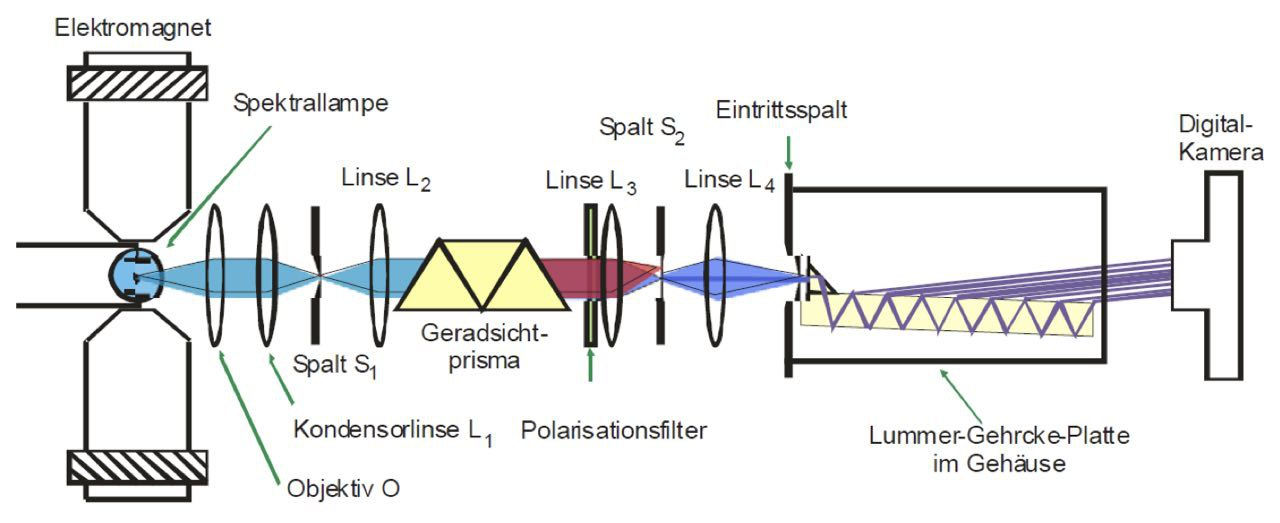
\includegraphics[width=0.7\textwidth]{bilder/aufbau.jpeg}
        \caption{Der schematische Aufbau des Versuchs ist hier dargestellt. \cite{anleitung}}
        \label{fig:aufbau}
    \end{figure}
    \FloatBarrier

    Eine Cadmium-Spektrallampe wird zwischen die Pole eines Elektromagneten gestellt.
    Das Licht senkrecht zum Magnetfeld soll im weiter Verlauf des Versuches betrachtet werden, weshalb der Strahlengang auch senkrecht zum Magnetfeld aufgebaut ist.
    Das ausgesandte Licht wird am Objektiv O kollimiert und danach durch die Kondensatorlinse L$_1$ auf den Spalt S$_1$ fokussiert.
    Weiterhin wird das Licht durch die Linse L$_2$ kollimiert und durch das Geradsichtprisma gesandt, welches das Licht, aufgrund verschiedener Brechungsindizes, der Wellenlänge nach aufspaltet.
    Ein Polarisationsfilter ermöglicht das Betrachten des zum Magnetfeld transversal und longitudinal polarisierten Lichtes.
    Nun kann das Licht durch die Linse L$_3$ so auf den Spalt S$_2$ abgebildet werden, dass nur eine bestimmte Wellenlänge durchgelassen wird und somit nur ein bestimmter Übergang betrachtet wird.
    Das wird erreicht, indem der Spalt senkrecht zum Strahlengang verschoben wird.
    Zum Schluss wird der Strahl durch die Linse L$_4$ auf den Eingang der Lummer-Gehrcke-Platte fokussiert, welche ein Interferenzmuster erzeugt.
    Mit einer Kamera werden Bilder aufgenommen und zur Bestimmung des Abstandes zwischen den Interferenzmaxima benutzt.

\subsection{Messung}
